\section{Asymmetrisk nøglekryptering og digitale certifikater}

\subsection{Læringsmål}

\begin{itemize}
	\item Redegør for og vis eksempler på asymmetrisk nøglekryptering, samt anvendelsen af
	asymmetrisk nøglekryptering på Internet.
	\item Samt forklar hvordan digitale certifikater udstedes og verificeres.
\end{itemize}

\subsection{Redegør for og vis eksempler på asymmetrisk nøglekryptering, samt anvendelsen af asymmetrisk nøglekryptering på Internet}
Figur~\ref{fig:asymmetrickeyenc} viser eksempel på asymmetrisk kryptering.

\begin{figure}[H]
	\centering
	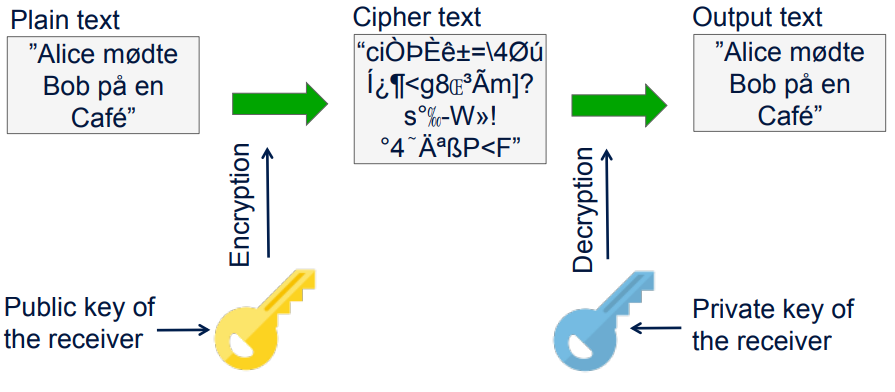
\includegraphics[width=0.7\linewidth]{figs/spm4/asymmetric_key_enc}
	\caption{Asymmetrisk kryptering}
	\label{fig:asymmetrickeyenc}
\end{figure}

\subsubsection{Matematikken}
Ligning~\ref{eq:asym} viser hvordan asymmetrisk kryptering virker. I ligningen er følgende forkortelser brugt: C: Ciphertext, P: Plaintext, E: Encryption rule, D: Decryption rule.

\begin{align}\label{eq:asym}
	C &= E(k_{priv}, P)\\
	P &= D(k_{priv}, E(k_{pub}, P))\\
	P &= D(k_{pub}, E(k_{priv}, P))
\end{align}

\subsubsection{Eksempel på RSA kryptering}
I Ligning~\ref{eq:rsa} er \textit{n} produktet af to primtal. Tallene \textit{d} og \textit{e} er primtallene.

\begin{align}\label{eq:rsa}
	Alice &= (n = 3233, e = 17)\\
	Bob &= (n = 3233, d = 413)\\
	Message &= 65\\
	Encrypted &= 65^{17}~mod~3233 = 2790\\
	Decrypted &= 2790^{413}~mod~3233 = 65
\end{align}

\subsubsection{Kryptering på internettet}
TLS er opgraderingen af SSL. Disse anvendes i \textit{transport} laget af netværkskommunikation. 

I applikationslaget hedder det \textit{HTTPS} når forbindelsen er beskyttet af TLS.

\subsection{Samt forklar hvordan digitale certifikater udstedes og verificeres}
Certifikater indeholder: en public key, en identitet og er signeret af en \textit{certificate authority}.

\subsubsection{Udstedelse}
Når et certifikat udsteder bruges flowet vist i Figur~\ref{fig:cert-issue}.

\begin{figure}[H]
	\centering
	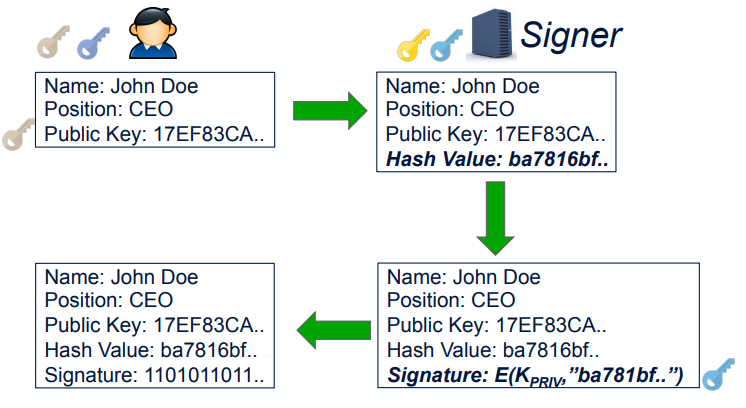
\includegraphics[width=0.75\linewidth]{figs/spm4/cert-issue}
	\caption{Udstedelse af et certifikat.}
	\label{fig:cert-issue}
\end{figure}

\subsubsection{Validering}
Ved validering af certifikater bruges flowt vist i Figur~\ref{fig:cert-validate}.

\begin{figure}[H]
	\centering
	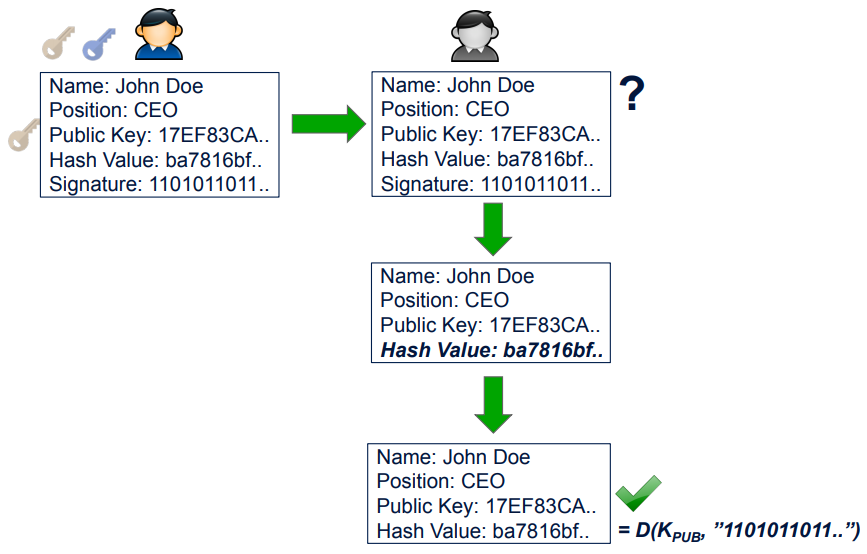
\includegraphics[width=0.85\linewidth]{figs/spm4/cert-validate}
	\caption{Validering af et certifikat.}
	\label{fig:cert-validate}
\end{figure}

